\documentclass[smallcondensed,referee]{svjour3}       % onecolumn (second format)
 \usepackage{textcomp} %for degree C
 \usepackage{url}
 \usepackage{amsmath}
 \usepackage{graphicx}
 \usepackage[authoryear]{natbib}
 \usepackage{lineno} 
 
\begin{document}
\title{How self-regulation, the storage effect and their interaction contribute
to coexistence in stochastic and seasonal environments}
\date{\today}
\author{Coralie Picoche$^{*,1}$ \and Fr\'ed\'eric Barraquand$^{1,2}$}
\titlerunning{Coexistence in seasonal environments}
\authorrunning{C.Picoche \& F.Barraquand}
\institute{{*}\email{coralie.picoche@u-bordeaux.fr}\\
$^{1}$ University of
Bordeaux, Integrative and Theoretical Ecology, LabEx COTE, B\^at. B2
- All\'ee Geoffroy St-Hilaire, 33615 Pessac, France \\
$^{2}$ CNRS, Institute
of Mathematics of Bordeaux, 351 Cours de la Lib\'eration, 33405 Talence,
France}
\journalname{Theoretical Ecology}

\maketitle
 
\linenumbers
\begin{abstract}
Explaining coexistence in species-rich communities of primary producers
remains a challenge for ecologists because of the likely competition
for shared resources. Following Hutchinson's seminal
suggestion, many theoreticians have tried to create diversity through
a fluctuating environment, which impairs or slows down competitive
exclusion. There are now several fluctuating-environment models allowing
coexistence, but they often produce only a dozen of coexisting species
at best. Here, we investigate how to create even richer communities
in fluctuating environments, using an empirically parameterized model.
Building on the forced Lotka-Volterra model of Scranton and Vasseur
(2016) inspired by phytoplankton communities, we have investigated
the effect of two coexistence mechanisms, namely the storage effect
and higher intra- than interspecific competition strengths (i.e.,
strong self-regulation). We tuned the competition ratio based on empirical
analyses, in which self-regulation usually dominates interspecific
interactions. Although a strong self-regulation maintained more species
(50\%) than the storage effect (25\%), we show that none of the two
coexistence mechanisms considered could, by itself, ensure the coexistence
of all species present at the beginning of our simulations. Realistic
seasonal environments only aggravated that picture, as they decreased
persistence relative to a random environment. Our results suggest
that combining different mechanisms for biodiversity maintenance into
community models might be more fruitful than trying to find which
mechanism explains best the observed diversity levels. We additionally
highlight that while trait-biomass distributions provide some clues
regarding coexistence mechanisms, they cannot indicate by themselves
which coexistence mechanisms are at play. \\
\textbf{Number of words: 242}\\
\textbf{Keywords: }coexistence; seasonality; competition; phytoplankton;
Lotka-Volterra; storage effect\\
\end{abstract}

\pagebreak{}
\section*{Introduction}

There has been a rich debate in theoretical ecology on how to reconcile
niche and neutral perspectives on species coexistence \citep{gravel_reconciling_2006,carmel_using_2017}.
Under the neutral perspective, all species have equal birth and death
rates and compete equally (since space is limited) whilst under the
niche perspective, birth and death rates can vary between species
and various mechanisms contribute to increasing intraspecific over
interspecific competition \citep{hubbell_unified_2001}. However,
as it has been pointed out repeatedly, niche and neutral processes
are not mutually exclusive: they may actually act together to produce
observed species coexistence \citep{gravel_reconciling_2006,mutshinda_what_2009,gotzenberger_ecological_2012}. 

An intriguing offshoot of the niche vs neutrality debate is the concept
of `clumpy coexistence' \citep{scheffer_self-organized_2006}, whereby
simultaneous influences of both niche and neutral processes create
several clumps of similar species along a single trait axis. Classical
stabilizing niche differences (SNDs), such as a net intraspecific
competition stronger than interspecific competition, enable coexistence
of multiple clumps \citep{chesson_mechanisms_2000}, while within-clump
coexistence occurs through neutral processes \citep{hubbell_unified_2001,munoz_neutral_2016},
as species that differ too little in their fitnesses cannot exclude
themselves out on reasonable timeframes. Indeed, clumps on the trait
axis eventually thin out in absence of immigration, but transient
coexistence can last for extended periods of time. This `emergent
neutrality' within groups \citep{holt_emergent_2006} has been proposed
as a unifying concept for the niche and neutral theories. The findings
of \citet{scheffer_self-organized_2006} have been disputed due to
hidden niches in the original model \citep{barabas_emergent_2013}.
Hidden niches emerge through stronger intraspecific competition mediated
by an additional predation-like term \citep{barabas_emergent_2013}.
This makes coexistence in the Scheffer and van Nes model more similar
to that of the classical Lotka-Volterra model \citep{barabas_effect_2016},
so that coexistence within clumps is not exactly neutral. Still, the
idea that niche and neutral assembly can mould communities stays potent
\citep{haegeman_mathematical_2011,vergnon_interpretation_2013}. Since
then, several studies have suggested that `clumpy coexistence' can
occur in theoretical models, most notably models incorporating temporal
variation \citep{scranton_coexistence_2016,sakavara_lumpy_2018}.
In these temporal-variation models, equal competitive strengths are
combined with other mechanisms like the storage effect (or temporal
niche partitioning, that is an equivalent concept for forced Lotka-Volterra
models, \citealp{barabas_community_2012,scranton_coexistence_2016}).
The storage effect increases the possibility of coexistence by making
the interaction strength covary positively with a fluctuating environmental
quality (see also \citealp{barabas_community_2012}). 

Here, we build on the work of \citet{scranton_coexistence_2016} to
investigate the possibility of coexistence through species response
to fluctuating environments. Our enthusiasm for the \citet{scranton_coexistence_2016}
model stems from our interest in phytoplankton communities, that inspired
their thermal preference curves modeling intrinsic growth rates. However,
\citet{scranton_coexistence_2016} described daily temperature as
a random noise, i.e., independent and identically distributed Gaussian
random variates over time. This appeared to us a key assumption to
relax. Under most latitudes, temperature is indeed a seasonal signal,
and seasonal forcing can strongly affect the dynamics of the community
considered \citep{vesipa_impact_2017}. Hence, over short timescales,
random temporal variations often only add noise to a largely deterministic
seasonal trend. Our present work can therefore be seen as an attempt
to blend \citet{scranton_coexistence_2016}'s stochastic framework
with the periodic environments of \citet{barabas_community_2012},
to better represent the mixture of stochastic and deterministic environmental
forces affecting phytoplankton community dynamics. 

Because many phytoplankton species or genera respond in similar ways
to temperature despite having different optimas \citep{moisan_modelling_2002},
we hypothesized that a large seasonal variation might not necessarily
foster species coexistence. In fact, similar responses to seasonal
fluctuations should lead to an increased synchrony of species abundances
which, in turn, should theoretically mitigate the expected temporal
partitioning. How seasonality affects coexistence (as opposed to a
purely randomly fluctuating environment) is therefore a key feature
of this paper. In particular, we contrast cases where the storage
effect is present vs absent, which conveniently maps to two different
parameterizations of the forced Lotka-Volterra model. Moreover, the
overall diversity obtained at the end of the simulations with \citet{scranton_coexistence_2016}'s
model was relatively low compared to what we usually observe in phytoplankton
communities (several dozens to hundreds of species). We have therefore
sought out which mechanisms would foster a truly species-rich community
for extended periods of time. 

In an empirical study combining phytoplankton community-level time
series and multivariate autoregressive models \citep{barraquand2018coastal},
we found that despite a large influence of the environment (including
temperature, irradiance, and other factors), a strong intraspecific
(or intragenus) competition, when compared to interspecific interaction
coefficients, was most likely the key driver of species coexistence.
In other words, strong self-regulation had a large role to play in
maintaining species diversity in coastal phytoplankton \citep{barraquand2018coastal}.
These high intraspecific interaction strengths mirror those found
in a number of terrestrial plant communities \citep{adler_competition_2018}
and in animal communities \citep{mutshinda_what_2009}.

Here, we therefore try to establish what are the relative contributions
to coexistence of the storage effect vs strong self-regulation, in
a phytoplankton-like theoretical community model. This led us to cross
different combinations of seasonality in the forcing signal, presence
of the storage effect or not, and intra- vs interspecific competition
intensity, in order to disentangle the contributions of all these
factors to biodiversity maintenance.
 
\section*{Methods}

\subsection*{\emph{Model description}}

The model described in \citet{scranton_coexistence_2016} is based
on the Lotka-Volterra competition model. Fluctuations in the environment
are introduced in the model by temperature-dependent intrinsic growth
rates (see Eq. \ref{eq:modelLV}-\ref{eq:growth}, all coefficients
are defined in Table \ref{tab:Coefficients-}) so that species growth
rates can be expressed as:

\begin{eqnarray}
\frac{dN_{i}}{dt} & = & r_{i}(\tau)N_{i}\left(1-\sum_{j=1}^{S}\alpha_{ij}N_{j}\right)-mN_{i}\label{eq:modelLV}\\
r_{i}(\tau) & = & a_{r}(\tau_{0})e^{E_{r}\frac{(\tau-\tau_{\text{0}})}{k\tau\tau_{0}}}f_{i}(\tau)\label{eq:growth}\\
\textnormal{where }f_{i}(\tau) & = & \begin{cases}
e^{-|\tau-\tau_{i}^{opt}|^{3}/b_{i}}, & \tau\leq\tau_{i}^{opt}\\
e^{-5|\tau-\tau_{i}^{opt}|^{3}/b_{i}}, & \tau>\tau_{i}^{opt}
\end{cases}\label{eq:eppley_curve}\\
\textnormal{and } b_{i}&\text{ such as} & \int r_{i}(\tau)d\tau=A\label{eq:niche_breadth}
\end{eqnarray}

Model parameters are detailed in Table \ref{tab:Coefficients-}, and
we set their values to match the features of phytoplankton communities
as in Scranton and Vasseur's work \citeyearpar{scranton_coexistence_2016}.
The niche of each species is defined by its thermal optimum $\tau_{i}^{opt}$.
Thermal performance curves defined in Eq. \ref{eq:eppley_curve} are
parameterized so that all species share the same niche area (Eq. \ref{eq:niche_breadth}),
which sets a trade-off between maximum growth rates and niche width. 

\begin{table}[!ht]
\centering{}%
\caption{Parameter definitions and values for the model described in Eqs. \ref{eq:modelLV}-\ref{eq:niche_breadth}.
Parameter values are not specified when they vary with time and/or
the species considered. \label{tab:Coefficients-}}
\begin{tabular}{ccc}
\hline 
Name & Definition & Value (unit)\\
\hline
$S$ & Initial number of species & 60 (NA)\\
$N_{i}$ & Biomass density of the $i^{th}$ species & (kg/area)\\
$\tau$  & Temperature & (K)\\
$r_{i}(\tau)$ & Growth rate of species $i$ as a function of temperature & $(\frac{\text{kg}}{\text{kg\ensuremath{\times}year}}$)\\
$\alpha_{ij}$ & Strength of competition of species $j\rightarrow i$  & 0.001 (area/kg)\\
$b_{i}$ & Normalization constant for the thermal decay rate & $(K^{3}$)\\
$m$ & Mortality rate & $15(\frac{\text{kg}}{\text{kg\ensuremath{\times}year}}$)\\
$\tau_{0}$ & Reference temperature & 293 (K) / 20 (\textdegree C)\\
$a_{r}(\tau_{0})$ & Growth rate at reference temperature & $386(\frac{\text{kg}}{\text{kg\ensuremath{\times}year}}$)\\
$E_{r}$ & Activation energy & 0.467 (eV)\\
$k$ & Boltzmann's constant & $8.6173324.10^{-5}(\text{eV.K}^{-1})$\\
$f_{i}(\tau)$ & Fraction of the maximum rate achieved for the $i^{th}$ species & (NA)\\
$\mu_{\tau}$ & Mean temperature & 293 (K)\\
$\sigma_{\tau}$ & Standard deviation for temperature & 5 (K)\\
$\tau_{\text{min}}$ & Minimum thermal optimum & 288 (K)\\
$\tau_{\text{max}}$ & Maximum thermal optimum & 298 (K)\\
A & Niche breadth & $10^{3.1}(\frac{\text{kg}}{\text{kg\ensuremath{\times}year}})$ \\
$\tau_{i}^{\text{opt}}$ & Thermal optimum for growth of the $i^{th}$ species & (K)\\
$\theta$ & Scaling between random and seasonal noise & (0;1.3) (NA)\\
$\kappa$ & Ratio of intra-to-interspecific competition strength & (1;10) (NA)\\
\hline
\end{tabular}
\end{table}
The original environmental forcing is a normally distributed variable
centered on 293 K (20\textdegree C), with a 5 K dispersion. Temperature varies
from one day to the next, but is kept constant throughout the day.
At the monthly or annual temporal scale usually used in ecological
studies, temperature could therefore be considered as a white noise
\citep{vasseur_color_2004}. However, from a mathematical viewpoint,
the noise is slightly autocorrelated as the integration process goes
below the daily time step. We therefore use the expression `random
noise' to describe this forcing, as opposed to the `seasonal noise'
described hereafter. To construct the seasonal noise, we add to the
random forcing signal a lower-frequency component, using a sinusoidal
function with a period of 365 days (Eq. \ref{eq:Seasonal_signal}).
We tune the ratio of low-to-high frequency with the variable $\theta$
so as to keep the same energy content - i.e., equal total variance
- in the forcing signal.

\begin{equation}
\tau(t)=\mu_{\tau}+\theta\sigma_{\tau}\sin\left(2\pi t\right)+\epsilon_{t},\text{where }\epsilon_{t}\sim\mathcal{N}\left(0,\sigma_{\tau}\sqrt{1-\frac{\theta^{2}}{2}}\right)\label{eq:Seasonal_signal}
\end{equation}

Note that the upper limit for $\theta$, $\sqrt{2}$, corresponds
to a completely deterministic model which we do not explore here (but
see \citet{zhao1991qualitative} proving bounded coexistence). We
choose to keep the stochasticity in the signal and to model a plausible
temperature signal with $\theta=1.3$ (illustrated in Fig. \ref{fig:Times-series_temperature_species}b)
when considering a seasonal forcing of the dynamics.

The formulation of the forced Lotka-Volterra model of \citet{scranton_coexistence_2016}
implies a storage effect, as the net effect of competition exerted
by species $j$ on $i$ is the product of the temperature-related
growth rate $r_{i}(\tau)$ and the competitive strength $\alpha_{ij}$
exerted by species $j$ multiplied by its abundance $N_{j}$. Therefore,
total net competition ($\sum_{j=1}^{S}r_{i}(\tau)\alpha_{ij}N_{j}$)
covaries positively with the growth rate values $r_{i}(\tau)$, which
defines the storage effect \citep{chesson_multispecies_1994,fox_intermediate_2013,ellner_how_2016}.
To remove the assumption of an explicit storage effect, we created
another version of the model using the mean value of a species' growth
rate ($\bar{r_{i}}$) to weight the interaction coefficients (see
Eq. \ref{eq:eqLV_noforcecompetition}). The mean growth rate value
was computed by first generating the temperature time series and then
averaging all $r_{i}$ over the corresponding sequences of $\tau$
values. 

\begin{equation}
\frac{dN_{i}}{dt}=N_{i}\left(r_{i}(\tau)-\sum_{j=1}^{S}\bar{r}_{i}\alpha_{ij}N_{j}\right)-mN_{i}\label{eq:eqLV_noforcecompetition}
\end{equation}

Following Eq. \ref{eq:eqLV_noforcecompetition}, net competition remains
unaffected by the environmental conditions, in contrast to intrinsic
growth rates, while preserving the same average magnitude as in Eq.
\ref{eq:modelLV}.

Strong self-regulation is ensured by the addition of the coefficient
$\kappa$, which is the ratio of intra-to-interspecific competition
strength. We can therefore re-write the interaction coefficients $\alpha_{ij}$
in Eq. \ref{eq:alpha_def}

\begin{equation}
\alpha_{ij}=\alpha\left(1+(\kappa-1)\delta_{ij}\right)\label{eq:alpha_def}
\end{equation}

where $\delta_{ij}$ is the Kronecker symbol, equal to 1 if $i=j$
and to 0 otherwise. The value of the parameter $\kappa=10$ was chosen
from analyses of phytoplanktonic data \citep{barraquand2018coastal}\footnote{The values of non-zero interspecific competition coefficients reported
in Fig. 5 of \citet{barraquand2018coastal} are somewhat higher than
here (and $\kappa$ lower, closer to 4) because the best-fitting model
actually set to zero some intergroup competition coefficients; using
a model where all $\alpha_{ij}$ are non-zero leads in contrast to
$\kappa=10$.}. Hereafter, the expression ``strong self-regulation'' characterizes
dynamics where the intraspecific competition strength is 10 times
higher than the interspecific competition strength, as opposed to
``equal competitive strengths'' where intra- and interspecific competition
strengths are equal. 

In addition to two types of environmental forcings (random noise with
$\theta=0$, and seasonal noise with $\theta=1.3$), we compare the
results for four formulations of the model: with and without an explicit
storage effect (Eq. \ref{eq:modelLV} and Eq. \ref{eq:eqLV_noforcecompetition},
respectively); with strong self-regulation or equal intra- and inter-competition
strength ($\kappa=10$ or $\kappa=1$, respectively). These are summed
up in Table \ref{tab:ModelsOfGrowthRates}.
\begin{center}
\begin{table}[!ht]
\begin{centering}
\caption{\label{tab:ModelsOfGrowthRates}Growth rate of species $i$ in the
four formulations of the model we present}
\begin{tabular}{ccc}
\hline 
$\frac{1}{N_{i}}\frac{dN_{i}}{dt}+m{}_{i}$ & Storage effect & No storage effect\\
\hline 
Strong self-regulation ($\kappa=10$) & $r_{i}(\tau)\left(1-\sum_{j=1}^{S}\alpha\left(1+9\delta_{ij}\right)N_{j}\right)$ & $r_{i}(\tau)-\sum_{j=1}^{S}\bar{r}_{i}\alpha\left(1+9\delta_{ij}\right)N_{j}$\\
Equal competitive strengths ($\kappa=1$) & $r_{i}(\tau)\left(1-\sum_{j=1}^{S}\alpha N_{j}\right)$ & $r_{i}(\tau)-\sum_{j=1}^{S}\bar{r}_{i}\alpha N_{j}$\\
\hline 
\end{tabular}
\par\end{centering}
\end{table}
\par\end{center}

\subsection*{\emph{Set-up}}

We replicate the `Species sorting' experiment of \citet{scranton_coexistence_2016}
so as to investigate how the structure of synthetic phytoplankton
communities varies under the different scenarios we described above.
We focused on the dynamics of a community initialized with 60 species
with thermal optima uniformly spaced along the interval {[}15\textdegree C, 25\textdegree C{]},
and with the same initial density $\left(\frac{\ensuremath{1}}{\alpha S}\right)$.
Each simulation was run for 5000 years in 1-day intervals. When the
density of a species dropped below $10^{-6}$, it was considered extinct.
For each combination of parameters (type of environmental signal,
storage effect and stabilizing niche differences), we ran 100 simulations. 

All simulations were run with Matlab's ode45 algorithm, an explicit
Runge-Kutta (4,5) integration scheme with an absolute error tolerance
of $10^{-8}$, and relative error tolerance of $10^{-3}$. The code
is available in a GitHub repository\footnote{\url{https://github.com/CoraliePicoche/Seasonality}, will be made
public upon acceptance or at the reviewer's request and stored in
Zenodo} .
 
\section*{Results}

\begin{figure}[!ht]
\begin{centering}
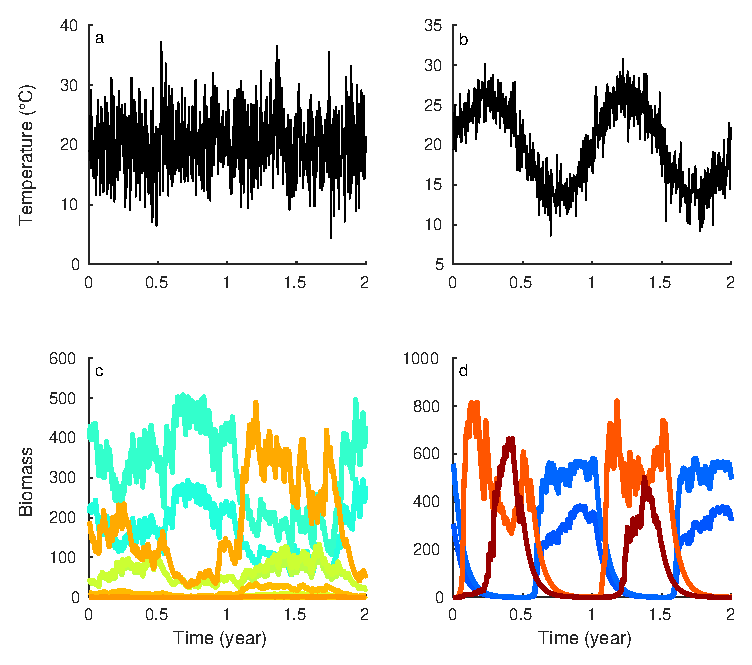
\includegraphics[width=0.95\textwidth]{Fig1}
\par\end{centering}
\caption{Time series of temperature (top; a-b) and extant species (bottom;
c-d) for the 2 last years of a 5000-year simulation, with storage
effect but no differences between intraspecific and interspecific
competition strengths. The forcing temperature is either a random
noise (a) or a seasonal noise (b), leading to community dynamics with
more erratic fluctuations (c) vs seasonally structured fluctuations
(d). Line colors of species biomasses correspond to their thermal
optimum (from blue, corresponding to low thermal optimum, to red,
corresponding to high thermal optimum).\label{fig:Times-series_temperature_species}}
\end{figure}

Typical dynamics of the community following Eq. \ref{eq:modelLV}
(the model of \citealp{scranton_coexistence_2016}), with both a purely
Gaussian noise (original choice of \citealp{scranton_coexistence_2016};
Fig. \ref{fig:Times-series_temperature_species}a) and a seasonal
noise described in Eq. \ref{eq:Seasonal_signal} (our variant, Fig.
\ref{fig:Times-series_temperature_species}b), are shown in Fig. \ref{fig:Times-series_temperature_species}c
and d, respectively. A sinusoidal forcing produces the strongly seasonally
structured dynamics that are typical of phytoplankton. Even though
only 5 species can be seen in Fig. \ref{fig:Times-series_temperature_species}c,
there were 14 species still present at the end of the simulation forced
by a random noise, with large disparities in the range of their biomasses.
A third of the species kept a biomass above 10 kg/area (setting area
= 1 ha, with a depth of a few meters, produces a realistic standing
biomasses; \citealp{reynolds2006ecology}) while 6 out of the 14 species
biomasses remained below the unit. All persisting species in the random
noise simulation were clustered within a 3.2\textdegree C-range of thermal optima
(see the biomass distribution as a function of the thermal optimum
in Supplementary Material, Fig. A1). No obvious temporal patterns
(e.g., cycles) could be seen in the community forced by random noise.
On the contrary, seasonal cycles were clear in the seasonally-forced
case of Fig. \ref{fig:Times-series_temperature_species}d. Only 4
species coexisted at the end of the simulation with seasonal noise,
gathered in two groups with large thermal optimum differences (5.7\textdegree C
between the maximum thermal optimum of the first group and the minimum
thermal optimum of the second group). When temperatures were high,
the group with higher thermal optima reached its maximum biomass,
then as temperature decreases through the season, these species leave
room for the growth of the low-temperature group.

\begin{figure}[!ht]
\begin{centering}
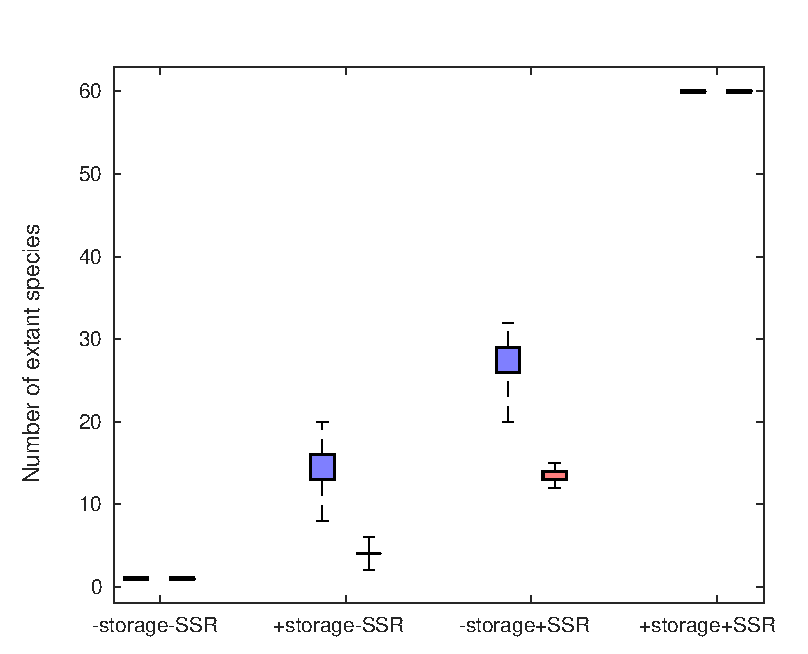
\includegraphics[width=0.75\textwidth]{Fig2}
\par\end{centering}
\caption{Number of species still present at the end of 100 simulations (5000
years each), initialized with 60 species, with a random forcing signal
(blue) or a seasonal noise (red). The signs + or -storage refer to
presence or absence of the storage effect, respectively; + / - SSR,
presence or absence of Strong Self-Regulation, respectively. Community
compositions are stable in the cases -storage-SSR and +storage+SSR,
for which 1 or 60 species are still present at the end of all simulations,
respectively. Due to low variance, the whiskers here represent min
and max rather than 1.5 interquartile range. \label{fig:Persistence-of-species} }
\end{figure}

The decrease in persistence due to seasonality observed in Fig. \ref{fig:Times-series_temperature_species}
was confirmed in all our simulations (Fig. \ref{fig:Persistence-of-species}).
In cases where final species richness varied from one simulation to
another (namely, the two middle cases in Fig. \ref{fig:Persistence-of-species}:
with storage effect but without strong self-regulation, or without
storage effect but with strong self-regulation), seasonality reduced
the number of extant species to, on average, 27\% and 48\% of their
original values, respectively (Fig. \ref{fig:Persistence-of-species}).
A seasonal signal therefore led to a much smaller average persistence.
There was also less variance in persistence between seasonally forced
simulations compared to random noise simulations. 

Both a strong self-regulation and the storage effect markedly increased
persistence. Without any of these coexistence mechanisms, only one
species persisted at the end of the simulations. When only the storage
effect was present, the number of extant species varied between 8
and 20 (14.8 $\pm$ 2.4) with random noise, or 2 and 6 (4.1 $\pm$
0.7) with a seasonal signal. On the other hand, when only a strong
self-regulation was present, the number of extant species nearly doubled,
varying between 20 and 32 (27.5 $\pm$ 2.4), or 12 and 15 (13.3 $\pm$
0.6), with a random or a seasonal noise, respectively. Remarkably,
when the storage effect and a strong self-regulation both affected
the community dynamics, all species persisted in the community, while
neither of these mechanisms was able to produce that result alone,
for either random and seasonal noise.

\begin{figure}[!ht]
\begin{centering}
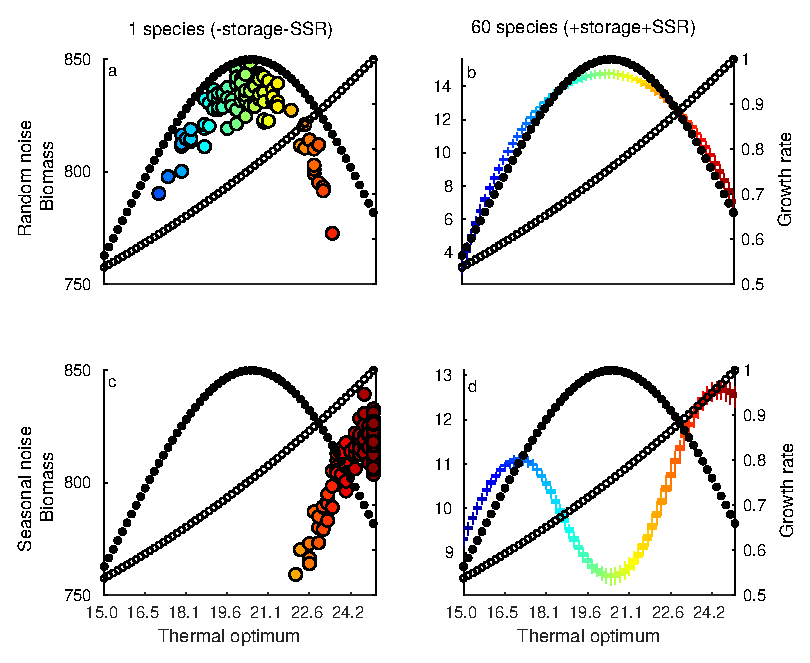
\includegraphics[bb=0bp 0bp 356bp 296bp,width=0.95\textwidth]{Fig3}
\par\end{centering}
\caption{Mean biomass distribution over the last 200 years for 100 simulations,
as a function of the species thermal optima. Here we consider the
two stable-composition cases and two types of forcing signal. On the
left column, simulations without storage effect nor strong self-regulation
are presented. Only one species is present at the end of the simulations
and its mean value is represented by one large colored circle per
simulation. There can be several circles for the same species, corresponding
to multiple simulations ending with this species alone. On the right
column, simulations with storage effect and strong self-regulation
are represented. All species are present at the end of the simulations
and small boxplots present the variation in the temporal average of
biomass with a given trait, for 100 simulations. The forcing signal
is either a random (top) or a seasonal noise (bottom). Each species
is identified by its thermal optimum through its color code. Scaled
(divided by maximum) average and maximum growth rates are shown as
small filled and open circles, respectively, and are indexed on the
right y-axis. \label{fig:Mean-biomass-in_stable_cases}}
\end{figure}

The trait-biomass distribution of the community was affected by the
type of forcing even when the richness of the community was stable
(Fig. \ref{fig:Mean-biomass-in_stable_cases}). Without storage effect
nor strong self-regulation, there was only one species left at the
end of the simulations. A random noise favored species with intermediate
thermal optima: the final species had a thermal optimum between 18.9\textdegree C
and 21.4\textdegree C (only a fourth of the initial range of thermal optima)
for two simulations out of three and the maximum final biomasses over
100 simulations was reached in this range (Fig. \ref{fig:Mean-biomass-in_stable_cases}a).
This distribution may indicate a selection for the highest long-term
growth rates, averaged over time (see scaled growth rates in Fig.
\ref{fig:Mean-biomass-in_stable_cases}). Seasonality with no coexistence
mechanisms also led to a single final species but, in this case, the
species always had a higher maximum growth rate (thermal optimum above
22\textdegree C). Species with a higher thermal optimum were more likely to persist
and to reach a higher biomass at the end of the simulation. 38\% of
the simulations therefore ended with the species having the highest
temperature optimum, 25\textdegree C. The shift in trait distribution towards
higher maximum growth rates with a seasonal noise vs higher average
growth rates with a random noise was consistent for all model types
considered. 

When both storage effect and strong self-regulation were present,
the 60 initial species coexisted with small variations in biomasses
for each species over the 100 simulations (mean CV=0.008 across simulations
with either a random or a seasonal noise, Fig. \ref{fig:Mean-biomass-in_stable_cases}b
and d). The forcing signal modified only the distribution of biomasses
resulting in contrasted community structures despite equal richness
in both simulation types. With a random noise, the distribution was
unimodal with a maximum biomass reached for the second highest long-term
average growth rate (corresponding to a thermal optimum of 20.2\textdegree C).
On the contrary, a seasonal signal led to a bimodal distribution (centered
on 17.0\textdegree C and 24.4\textdegree C), each corresponding to one season, with highest
biomasses for higher thermal optima (Fig. \ref{fig:Mean-biomass-in_stable_cases}d).
The minimum biomass was reached for the highest long-term average
growth rate at an intermediate temperature (20.4\textdegree C).

\begin{figure}[!ht]
\begin{centering}
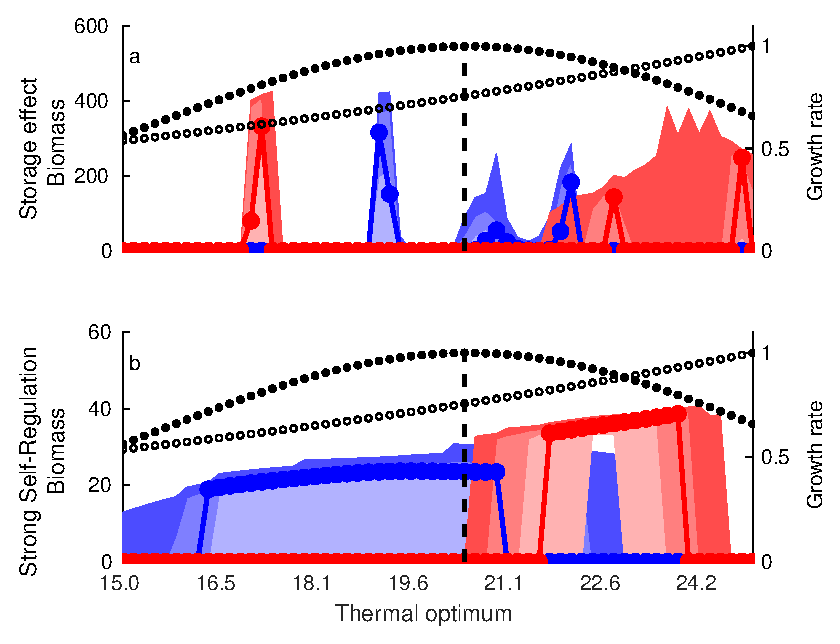
\includegraphics[bb=0bp 0bp 428bp 338bp,width=0.85\textwidth]{Fig4}
\par\end{centering}
\caption{Mean biomass distribution over the last 200 years for 100 simulations,
as a function of thermal optima, with storage effect and equal competitive
strengths (a) and without storage effect, with strong self-regulation
(b). The forcing signal is either a random (in blue) or a seasonal
noise (in red). Shades of the same color correspond to the 50th, 90th
and 100th percentiles of the distributions while colored lines correspond
to one representative simulation. Scaled (divided by maximum) average
(whose maximum is indicated by the dashed line) and maximum growth
rates are shown as filled and open and circles, respectively, and
indexed on the right y-axis. \label{fig:Unstable_cases}}
\end{figure}

In cases where the richness of the community varied, the overall shape
(multimodal vs unimodal) of the marginal distribution of extant species
with respect to the trait axis were similar for both types of environmental
forcings (Fig. \ref{fig:Unstable_cases}). By contrast, the type of
coexistence mechanism generated different shapes. Indeed, the storage
effect (when acting alone) led to a multimodal biomass distribution
with respect to thermal optima. We always observed 3 modes with a
random noise and 3 modes in 95\% of the seasonal simulations (Fig.
\ref{fig:Unstable_cases}a). With a random noise, extant species were
grouped in rather similar clumps regarding species thermal optima
(between 18.8\textdegree C and 22.2\textdegree C) whereas species tended to be further apart
in the seasonal case, covering a total range of 7.7\textdegree C, with species
grouping in the higher part of the thermal range, above 22\textdegree C. On the
other hand, strong self-regulation led to a quasi-uniform biomass
distribution (Fig. \ref{fig:Unstable_cases} b). Species in communities
forced by a random noise stayed in the lower range of thermal optima
(in 96\% of the simulations, the highest thermal optimum was 22.4\textdegree C,
see Fig. A2 in the Supplementary Material) while they were filtered
out in communities subjected to a seasonal fluctuation of their environment,
for which species with thermal optima above 20.5\textdegree C persisted. As before
(Fig. \ref{fig:Mean-biomass-in_stable_cases}), seasonality promoted
species with a higher maximum growth rate since the autocorrelated
temperatures enabled them to achieve this highest growth rate for
a longer period of time than a random noise would have. 

\section*{Discussion}

We have simulated competitive Lotka-Volterra dynamics forced by a
fluctuating environment (e.g., temperature fluctuations) under a range
of scenarios allowing more or less coexistence. Two coexistence mechanisms,
the storage effect and strong self-regulation (i.e., intraspecific
competition much stronger than interspecific competition), could be
either present or absent, which led to four scenarios. These four
scenarios were crossed with two possibilities for the forcing signal,
a random noise (mostly white) and a stochastic yet seasonal signal,
both with equal temporal variance. Our investigation therefore built
on the model of \citet{scranton_coexistence_2016}, which included
a random forcing and a storage effect, but considered seven additional
combinations of mechanisms. This was motivated by our wish to include
two observed features of phytoplankton dynamics: seasonal cycles \citep{winder_annual_2010}
and strong self-regulation \citep{chesson_mechanisms_2000,adler_coexistence_2010,barraquand2018coastal}.
Many mechanisms can lead to intraspecific competition being stronger
than interspecific competition: nonlinearities in the functional forms
of competition or mutualism that contribute to increasing self-regulation
\citep{kawatsu2018density}, or predation as well as parasitism (see
e.g., the generalist predators in \citealp{haydon1994pivotal}). Strong
self-regulation seems nonetheless an ubiquitous feature in competition
networks of primary producers \citep{adler_competition_2018}, and
perhaps even more general networks \citep{barabas_self-regulation_2017}.

Before discussing the ecological interpretation of our results, we
first recall some technical assumptions made in this study. All our
simulations lasted for a fixed duration (5000 timesteps) as in \citet{scranton_coexistence_2016}.
This means that short- and medium-term transients (a few years to
hundreds of years) are completely negligible at the end of the time
series, but very long transients can remain. We realized that convergence
could be incomplete after 5000 years in some cases (e.g., random noise
+ storage effect + equal competitive strength). Such simulations would
take up to 15 000 years to converge and the rate of convergence would
slow over time, as can also be observed for similar models \citep{scheffer_self-organized_2006}.
We kept a fixed time integration window rather than waiting for convergence
for both technical and ecological reasons. From a technical standpoint,
adding 10 000 years of numerical integration (or more) for the sake
of reaching equilibrium would have been very challenging computationally,
and comparison with the values reported by \citet{scranton_coexistence_2016}
would have been compromised. From an ecological standpoint, waiting
for full convergence when there are extremely long transients \citep{hastings_transient_2018}
is also quite artificial: there is no reason to believe that very
long transients (i.e., transients that maintains for thousands of
years) have any less ecological reality than an attractor that is
deemed stable. Speed of convergence is therefore an issue to judge
whether transients should be considered or excluded, and a very long
yet fixed time window for integration allows advantageously to compare
all mechanisms. 

Another assumption pertains to competition coefficients. To allow
for comparison with \citet{scranton_coexistence_2016}, we did not
introduce variability in intraspecific competition strength or interspecific
competition strength. By contrast, data-based coefficients vary between
species \citep{barraquand2018coastal}, with a majority of weak interactions
(as suggested in \citealp{wootton_measurement_2005}) and more variance
in intraspecific coefficients. \citet{stump_multispecies_2017} recently
considered the potential effects of competition coefficient variability
(also called non-diffuse competition), as did \citet{kokkoris_variability_2002};
more variance in interspecific competition strength is usually detrimental
to coexistence (see \citet{stump_multispecies_2017} for a classification
of the various effects). Setting the competition coefficients using
a multidimensional trait-based framework, like that of \citet{ashby_competing_2017},
would provide a natural development to the work presented here; it
is in our opinion difficult to speculate on those variance effects
because both intra- and interspecific competition coefficient variances
may matter to community persistence. 

Finally, our study is limited to communities whose species have fast
population dynamics relative to the yearly timescale, like phytoplankton
and likely other fast-living organisms, so that many generations can
occur in a year. Different effects of seasonality may occur in species
that have slower life histories or with generations that extend over
multiple years (e.g., multiyear cycles and chaotic attractors, \citealt{rinaldi_multiple_1993,taylor_how_2013,tyson_seasonally_2016}).
Persistence may be affected differently by seasonality in such cases
with slower community dynamics. 

With these assumptions in mind, we have found that first, temporally
forced Lotka-Volterra dynamics cannot sustain any diversity with our
phytoplankton-based set of parameters, unless the structure is geared
to include either a storage effect or a strong self-regulation. Although
this absence of diversity-enhancing effect of ``pure'' environmental
variation has already been stated by other authors \citep{chesson_roles_1997,barabas_community_2012,fox_intermediate_2013,scranton_coexistence_2016},
this is not always intuitive \citep{fox_intermediate_2013}, so we
feel compelled to stress it once more: temporal variation in growth
rate alone cannot help coexistence within competitive communities.
A nice point made by \citet{scranton_coexistence_2016} was that a
built-in storage effect in a forced Lotka-Volterra model, parameterized
for phytoplankton communities, could lead to some degree of coexistence.
Our investigation reproduced these results, using the random noise
considered by \citet{scranton_coexistence_2016}. However, an arguably
more lifelike noisy and seasonal temperature forcing considerably
lessened the richness of the community after 5000 years, decreasing
from 15 to 4 species on average. Even imagining that groups represented
here are genera or classes rather than species, this is a fairly low
diversity for a phytoplankton-like community (see e.g., Chapter 1
in \citealp{reynolds2006ecology}). This suggests that the storage
effect may not, on its own, be sufficient to maintain species-rich
communities (e.g., dozens to hundreds of species). We have therefore
sought out whether a stronger self-regulation could maintain a higher
diversity, using field-based intra- vs intergroup (species or genera)
competition strength ratio \citep{barraquand2018coastal}, where the
intragroup density-dependence was estimated 10 times stronger. Implementing
such strong self-regulation, in the forced Lotka-Volterra models that
we considered, produced a higher level of diversity than the storage
effect (almost double). Of course, the result is somehow contingent
upon the strength of self-regulation. Our estimates are a little stronger
than what was found in perennial plants \citep{adler_coexistence_2010},
where interspecific competition was suggested 4 or 5 times stronger
than intraspecific. Still, the widespread effects of natural enemies
in phytoplankton (zooplankton, parasites) may contribute to increase
the strength of self-regulation \citep{barraquand2018coastal,chesson_updates_2018}
relative to other systems, hence we believe that 10 times stronger
intraspecific competition constitutes a reasonable order of magnitude. 

However, such strong self-regulation was still insufficient to maintain
the whole community diversity (60 species) by itself, especially when
the seasonal forcing (always decreasing species richness) was considered.
The diversity within clumps of similar values of thermal optima was
considerably decreased once seasonality was implemented. This diversity
reduction occurs because within a season, the signal autocorrelation
gives long, contiguous time intervals to the best competitor to exclude
its less adapted competitors. This makes the results likely to hold
not only for seasonal environments, but more generally for autocorrelated
ones above the daily scale, i.e., ``red'' noise. In contrast, the
random noise scenario -- which can be considered white noise above
the daily temporal scales -- generates large temperature shifts more
frequently, and thereby forbids such competitive exclusion. In a seasonal
setting, a species with the highest long-term (arithmetically) averaged
growth rate may not be the best competitor, and can disappear as a
result of a strong competition from both low- and high-temperature
tolerant species. This holds with or without a storage effect. 

Our results may appear at odds with recent proposals that seasonal
forcing in itself would help maintain diversity \citep{sakavara_lumpy_2018}.
However, we compared the effect of seasonal forcing to that of other
forcing signals while controlling for total variance. Thus, the contrast
between our results and those of \citet{sakavara_lumpy_2018} may
be due to the role of forcing variance over time (we compare scenarios
under a constant total variance). Overall, while seasonality may be
slightly better than no forcing at all in maintaining diversity if
a storage effect is present, seasonal forcing of parameters does not
improve coexistence when compared to white noise.

In addition to community diversity, the biomass-trait relationship
also varied from one simulation to another. Some regularities did
emerge across simulations though. The storage effect begot several
clumps along the trait space (as observed by \citealp{scranton_coexistence_2016}).
The seasonality that we added to the temperature signal led to more
distant clumps on the trait axis, with less species per clump. Conversely,
strong self-regulatory mechanisms alone led to relatively uniform
biomass distributions, with species forming a single large cluster,
which covers a fraction of the initial trait space. Therefore, the
shape of the distribution was affected by the coexistence mechanism
at work while the average trait value was modified by the type of
environmental forcing, even though the mean value of the environmental
signal did not change. The biomass-trait distributions therefore constitute
clues to interpret community dynamics \citep{dandrea_challenges_2016,loranger_what_2018},
although we certainly recommend to interpret them with caution to
avoid over-generalization. The identification of multiple modes in
biomass-trait relationships and SADs is relatively recent \citep{dornelas_multiple_2008,matthews_multimodal_2014}
and is a rare pattern in theoretical models \citep{mcgill_species_2007}.
\citet{barabas_emergent_2013} convincingly argued that multimodality
could arise from the demographic stochasticity of a single model run
(with either self-regulation or neutrality, but without the clumpy
coexistence emerging from a storage effect). However, our results
are based on many model runs, for which either the storage effect
alone or a storage effect + strong self-regulation in a seasonal context
consistently produced multimodal distributions, while simulations
without the storage effect always led to a single cluster along the
trait axis. Our suggestion for empirical studies is as follows: if
only one spatial location is observed, caution in interpreting multiple
clumps on the trait axis is of course required, as \citet{barabas_emergent_2013}
highlighted. However, with several locations - or in a theoretical
context - one could average across locations to reproduce similar
graphs to the ones produced here. Clumps in the trait axis when averaged
across model runs/locations are therefore a signature of a coexistence
induced by the storage effect, for the cases that we considered in
the article. Of course, other mechanisms that we did not include in
our models may produce similar patterns \citep{rael2018emergent}
or obfuscate these patterns -- typically strong self-regulation weakens
the clustering on the trait axis. We therefore view clustering on
the trait axis (when averaged over several samples) as an interesting
clue suggesting to look for a storage effect, rather than any definite
proof that the storage effect is at work. 

In our previous empirical study of coastal phytoplankton dynamics
\citep{barraquand2018coastal}, we did not find any storage effect.
This, however, does not mean that it could not be observed in other
planktonic systems. Given the consequences of the storage effect for
species richness and composition presented here, we are skeptical
that the storage effect could by itself help explaining phytoplankton
diversity. However, our results suggest that in phytoplankton-like
seasonal environments, even though empirically-based self-regulation
produce much more diversity than the storage effect when considered
in isolation, the storage effect can help diversity maintenance when
combined to other mechanisms. Indeed, the combination storage effect
+ strong self-regulation is non-additive: the cases were both self-regulation
and the storage effect were present showed more diversity than generated
by any mechanism on its own. 

The above results suggest the very exciting idea that multiple coexistence
mechanisms might combine superadditively, thus helping us to better
understand the astounding diversity of primary producers. This logic
could, in principle, be extended to mechanisms that we have not considered
here (e.g., spatial structure, specialized natural enemies, that could
be as important here for plankton as they are for tropical trees,
see \citealp{bagchi_pathogens_2014,comita_testing_2014,barraquand2018coastal}).
Previous research has however demonstrated that generalist seed predation
could weaken the storage effect \citep{kuang_coexistence_2009,kuang_interacting_2010}
thus different mechanisms might not always combine superadditively
as we found here. That said, superadditivity has been found in some
cases, i.e., pathogens could enhance the storage effect \citep{mordecai_pathogen_2015}.
Better explaining plant or microbial diversity would then not be about
selecting the best unique mechanism susceptible to explain the observed
diversity, but rather better combining those mechanisms together.
This may obviously be an annoyance for those who like to sharpen Occam's
razor, but it clearly holds opportunities for theoreticians wishing
to investigate synergies between coexistence mechanisms in highly
diverse communities. Aside from the synergies between predator diversity-enhancing
effects, strong self-regulation through various means and storage
effects (on the temporal axis), one obvious follow-up of this research
would be interactions with spatial structure. Spatial structure occurs
both endogeneously, through spatially restricted movements and interactions,
and exogeneously, through spatial variation in environmental covariates
\citep{bolker_combining_2003}. Numerous studies \citep[e.g.,][]{bolker_spatial_1999,murrell_2002}
have shown that spatially restricted movements and interactions -
very small-scale spatial structure - can help coexistence, which we
believe would be especially important for phytoplankton since many
species form colonies (\citealp{reynolds2006ecology}; see discussion
in \citealp{barraquand2018coastal}). Moreover, although temperature
is usually relatively spatially homogeneous over space, other drivers
(e.g., rainfall, pH in terrestrial ecosystems; salinity in aquatic
ones) may exhibit spatial variation which is a main factor for coexistence
\citep{snyder_when_2008}. The odds that different (resource) niches,
natural enemies, spatial limits to competition and temporal niche
partitioning all interact to promote the very high-dimensional coexistence
observed in the field seem much higher than for any of those mechanisms
alone. Whether the diversity-enhancing effects of these mechanisms
combine subadditively (as in \citealp{kuang_interacting_2010}) or
superadditively like here is therefore worthy of further research. 

\begin{acknowledgements} 
We thank Alix Sauve for thoughtful comments and some bibliographic
references, as well as Gy\"orgy Barab\'as and an anonymous referee for
constructive feedback. This study was supported by the French ANR
through LabEx COTE (ANR-10-LABX-45).
\end{acknowledgements}
% 
\begin{thebibliography}{56}
\providecommand{\natexlab}[1]{#1}
\providecommand{\url}[1]{{#1}}
\providecommand{\urlprefix}{URL }
\expandafter\ifx\csname urlstyle\endcsname\relax
  \providecommand{\doi}[1]{DOI~\discretionary{}{}{}#1}\else
  \providecommand{\doi}{DOI~\discretionary{}{}{}\begingroup
  \urlstyle{rm}\Url}\fi
\providecommand{\eprint}[2][]{\url{#2}}

\bibitem[{Adler et~al.(2010)Adler, Ellner, and Levine}]{adler_coexistence_2010}
Adler PB, Ellner SP, Levine JM (2010) Coexistence of perennial plants: an
  embarrassment of niches. Ecology letters 13(8):1019--1029,
  \doi{10.1111/j.1461-0248.2010.01496.x}

\bibitem[{Adler et~al.(2018)Adler, Smull, Beard, Choi, Furniss, Kulmatiski,
  Meiners, Tredennick, and Veblen}]{adler_competition_2018}
Adler PB, Smull D, Beard KH, Choi RT, Furniss T, Kulmatiski A, Meiners JM,
  Tredennick AT, Veblen KE (2018) Competition and coexistence in plant
  communities: intraspecific competition is stronger than interspecific
  competition. Ecology Letters 21(9):1319--1329, \doi{10.1111/ele.13098}

\bibitem[{Ashby et~al.(2017)Ashby, Watkins, Louren\c{c}o, Gupta, and
  Foster}]{ashby_competing_2017}
Ashby B, Watkins E, Louren\c{c}o J, Gupta S, Foster KR (2017) Competing species
  leave many potential niches unfilled. Nature Ecology \& Evolution
  1(10):1495--1501, \doi{10.1038/s41559-017-0295-3}

\bibitem[{Bagchi et~al.(2014)Bagchi, Gallery, Gripenberg, Gurr, Narayan, Addis,
  Freckleton, and Lewis}]{bagchi_pathogens_2014}
Bagchi R, Gallery RE, Gripenberg S, Gurr SJ, Narayan L, Addis CE, Freckleton
  RP, Lewis OT (2014) Pathogens and insect herbivores drive rainforest plant
  diversity and composition. Nature 506(7486):85--88, \doi{10.1038/nature12911}

\bibitem[{Barab\'as et~al.(2012)Barab\'as, Mesz\'ena, and
  Ostling}]{barabas_community_2012}
Barab\'as G, Mesz\'ena G, Ostling A (2012) Community robustness and limiting
  similarity in periodic environments. Theoretical Ecology 5(2):265--282,
  \doi{10.1007/s12080-011-0127-z}

\bibitem[{Barab\'as et~al.(2013)Barab\'as, D'Andrea, Rael, Mesz\'ena, and
  Ostling}]{barabas_emergent_2013}
Barab\'as G, D'Andrea R, Rael R, Mesz\'ena G, Ostling A (2013) Emergent
  neutrality or hidden niches? Oikos 122(11):1565--1572,
  \doi{10.1111/j.1600-0706.2013.00298.x}

\bibitem[{Barab\'as et~al.(2016)Barab\'as, Michalska-Smith, and
  Allesina}]{barabas_effect_2016}
Barab\'as G, Michalska-Smith MJ, Allesina S (2016) The {Effect} of {Intra}- and
  {Interspecific} {Competition} on {Coexistence} in {Multispecies}
  {Communities}. The American Naturalist 188(1):E1--E12, \doi{10.1086/686901}

\bibitem[{Barab\'as et~al.(2017)Barab\'as, Michalska-Smith, and
  Allesina}]{barabas_self-regulation_2017}
Barab\'as G, Michalska-Smith MJ, Allesina S (2017) Self-regulation and the
  stability of large ecological networks. Nature Ecology \& Evolution
  1(12):1870--1875, \doi{10.1038/s41559-017-0357-6}

\bibitem[{Barraquand et~al.(2018)Barraquand, Picoche, Maurer, Carassou, and
  Auby}]{barraquand2018coastal}
Barraquand F, Picoche C, Maurer D, Carassou L, Auby I (2018) Coastal
  phytoplankton community dynamics and coexistence driven by intragroup
  density-dependence, light and hydrodynamics. Oikos In press,
  \doi{10.1101/171264}

\bibitem[{Bolker and Pacala(1999)}]{bolker_spatial_1999}
Bolker B, Pacala S (1999) Spatial {Moment} {Equations} for {Plant}
  {Competition}: {Understanding} {Spatial} {Strategies} and the {Advantages} of
  {Short} {Dispersal}. The American Naturalist 153(6):575--602,
  \doi{10.1086/303199}

\bibitem[{Bolker(2003)}]{bolker_combining_2003}
Bolker BM (2003) Combining endogenous and exogenous spatial variability in
  analytical population models. Theoretical Population Biology 64(3):255--270,
  \doi{10.1016/S0040-5809(03)00090-X}

\bibitem[{Carmel et~al.(2017)Carmel, Suprunenko, Kunin, Kent, Belmaker,
  Bar-Massada, and Cornell}]{carmel_using_2017}
Carmel Y, Suprunenko YF, Kunin WE, Kent R, Belmaker J, Bar-Massada A, Cornell
  SJ (2017) Using exclusion rate to unify niche and neutral perspectives on
  coexistence. Oikos 126(10):1451--1458, \doi{10.1111/oik.04380}

\bibitem[{Chesson(1994)}]{chesson_multispecies_1994}
Chesson P (1994) Multispecies {Competition} in {Variable} {Environments}.
  Theoretical Population Biology 45:227--276, \doi{10.1006/tpbi.1994.1013}

\bibitem[{Chesson(2000)}]{chesson_mechanisms_2000}
Chesson P (2000) Mechanisms of maintenance of species diversity. Annual review
  of Ecology and Systematics 31:343--366,
  \doi{10.1146/annurev.ecolsys.31.1.343}

\bibitem[{Chesson(2018)}]{chesson_updates_2018}
Chesson P (2018) Updates on mechanisms of maintenance of species diversity.
  Journal of Ecology 106(5):1773--1794, \doi{10.1111/1365-2745.13035}

\bibitem[{Chesson and Huntly(1997)}]{chesson_roles_1997}
Chesson P, Huntly N (1997) The roles of harsh and fluctuating conditions in the
  dynamics of ecological communities. The American Naturalist 150(5):519--553,
  \doi{10.1086/286080}

\bibitem[{Comita et~al.(2014)Comita, Queenborough, Murphy, Eck, Xu, Krishnadas,
  Beckman, and Zhu}]{comita_testing_2014}
Comita LS, Queenborough SA, Murphy SJ, Eck JL, Xu K, Krishnadas M, Beckman N,
  Zhu Y (2014) {Testing predictions of the Janzen-Connell hypothesis: a
  meta-analysis of experimental evidence for distance- and density-dependent
  seed and seedling survival}. Journal of Ecology 102(4):845--856,
  \doi{10.1111/1365-2745.12232}

\bibitem[{D'Andrea and Ostling(2016)}]{dandrea_challenges_2016}
D'Andrea R, Ostling A (2016) Challenges in linking trait patterns to niche
  differentiation. Oikos 125(10):1369--1385, \doi{10.1111/oik.02979}

\bibitem[{Dornelas and Connolly(2008)}]{dornelas_multiple_2008}
Dornelas M, Connolly SR (2008) Multiple modes in a coral species abundance
  distribution. Ecology Letters 11(10):1008--1016,
  \doi{10.1111/j.1461-0248.2008.01208.x}

\bibitem[{Ellner et~al.(2016)Ellner, Snyder, and Adler}]{ellner_how_2016}
Ellner SP, Snyder RE, Adler PB (2016) How to quantify the temporal storage
  effect using simulations instead of math. Ecology Letters 19(11):1333--1342,
  \doi{10.1111/ele.12672}

\bibitem[{Fox(2013)}]{fox_intermediate_2013}
Fox JW (2013) The intermediate disturbance hypothesis should be abandoned.
  Trends in Ecology \& Evolution 28(2):86--92, \doi{10.1016/j.tree.2012.08.014}

\bibitem[{G\"{o}tzenberger et~al.(2012)G\"{o}tzenberger, de~Bello, Br\r{a}then,
  Davison, Dubuis, Guisan, Lep\v{s}, Lindborg, Moora, P\"{a}rtel, Pellissier,
  Pottier, Vittoz, Zobel, and Zobel}]{gotzenberger_ecological_2012}
G\"{o}tzenberger L, de~Bello F, Br\r{a}then KA, Davison J, Dubuis A, Guisan A,
  Lep\v{s} J, Lindborg R, Moora M, P\"{a}rtel M, Pellissier L, Pottier J,
  Vittoz P, Zobel K, Zobel M (2012) Ecological assembly rules in plant
  communities-approaches, patterns and prospects. Biological Reviews
  87(1):111--127, \doi{10.1111/j.1469-185X.2011.00187.x}

\bibitem[{Gravel et~al.(2006)Gravel, Canham, Beaudet, and
  Messier}]{gravel_reconciling_2006}
Gravel D, Canham CD, Beaudet M, Messier C (2006) Reconciling niche and
  neutrality: the continuum hypothesis: {Reconciling} niche and neutrality.
  Ecology Letters 9(4):399--409, \doi{10.1111/j.1461-0248.2006.00884.x}

\bibitem[{Haegeman and Loreau(2011)}]{haegeman_mathematical_2011}
Haegeman B, Loreau M (2011) A mathematical synthesis of niche and neutral
  theories in community ecology. Journal of Theoretical Biology
  269(1):150--165, \doi{10.1016/j.jtbi.2010.10.006}

\bibitem[{Hastings et~al.(2018)Hastings, Abbott, Cuddington, Francis, Gellner,
  Lai, Morozov, Petrovskii, Scranton, and Zeeman}]{hastings_transient_2018}
Hastings A, Abbott KC, Cuddington K, Francis T, Gellner G, Lai YC, Morozov A,
  Petrovskii S, Scranton K, Zeeman ML (2018) Transient phenomena in ecology.
  Science 361(6406):eaat6412, \doi{10.1126/science.aat6412}

\bibitem[{Haydon(1994)}]{haydon1994pivotal}
Haydon D (1994) Pivotal assumptions determining the relationship between
  stability and complexity: an analytical synthesis of the stability-complexity
  debate. The American Naturalist 144(1):14--29, \doi{10.1086/285658}

\bibitem[{Holt(2006)}]{holt_emergent_2006}
Holt R (2006) Emergent neutrality. Trends in Ecology \& Evolution
  21(10):531--533, \doi{10.1016/j.tree.2006.08.003}

\bibitem[{Hubbell(2001)}]{hubbell_unified_2001}
Hubbell SP (2001) The {Unified} {Neutral} {Theory} of {Biodiversity} and
  {Biogeography} ({MPB}-32). Princeton University Press

\bibitem[{Kawatsu and Kondoh(2018)}]{kawatsu2018density}
Kawatsu K, Kondoh M (2018) Density-dependent interspecific interactions and the
  complexity--stability relationship. Proc R Soc B 285(1879):20180698,
  \doi{10.1098/rspb.2018.0698}

\bibitem[{Kokkoris et~al.(2002)Kokkoris, Jansen, Loreau, and
  Troumbis}]{kokkoris_variability_2002}
Kokkoris GD, Jansen VAA, Loreau M, Troumbis AY (2002) Variability in
  interaction strength and implications for biodiversity. Journal of Animal
  Ecology 71(2):362--371, \doi{10.1046/j.1365-2656.2002.00604.x}

\bibitem[{Kuang and Chesson(2009)}]{kuang_coexistence_2009}
Kuang JJ, Chesson P (2009) Coexistence of annual plants: generalist seed
  predation weakens the storage effect. Ecology 90(1):170--182,
  \doi{10.1890/08-0207.1}

\bibitem[{Kuang and Chesson(2010)}]{kuang_interacting_2010}
Kuang JJ, Chesson P (2010) Interacting coexistence mechanisms in annual plant
  communities: frequency-dependent predation and the storage effect.
  Theoretical population biology 77(1):56--70, \doi{10.1016/j.tpb.2009.11.002}

\bibitem[{Loranger et~al.(2018)Loranger, Munoz, Shipley, and
  Violle}]{loranger_what_2018}
Loranger J, Munoz F, Shipley B, Violle C (2018) What makes trait-abundance
  relationships when both environmental filtering and stochastic neutral
  dynamics are at play? Oikos \doi{10.1111/oik.05398}

\bibitem[{Matthews et~al.(2014)Matthews, Borges, and
  Whittaker}]{matthews_multimodal_2014}
Matthews TJ, Borges PAV, Whittaker RJ (2014) Multimodal species abundance
  distributions: a deconstruction approach reveals the processes behind the
  pattern. Oikos 123(5):533--544, \doi{10.1111/j.1600-0706.2013.00829.x}

\bibitem[{McGill et~al.(2007)McGill, Etienne, Gray, Alonso, Anderson, Benecha,
  Dornelas, Enquist, Green, He, Hurlbert, Magurran, Marquet, Maurer, Ostling,
  Soykan, Ugland, and White}]{mcgill_species_2007}
McGill BJ, Etienne RS, Gray JS, Alonso D, Anderson MJ, Benecha HK, Dornelas M,
  Enquist BJ, Green JL, He F, Hurlbert AH, Magurran AE, Marquet PA, Maurer BA,
  Ostling A, Soykan CU, Ugland KI, White EP (2007) Species abundance
  distributions: moving beyond single prediction theories to integration within
  an ecological framework. Ecology Letters 10(10):995--1015,
  \doi{10.1111/j.1461-0248.2007.01094.x}

\bibitem[{Moisan et~al.(2002)Moisan, Moisan, and
  Abbott}]{moisan_modelling_2002}
Moisan JR, Moisan TA, Abbott MR (2002) Modelling the effect of temperature on
  the maximum growth rates of phytoplankton populations. Ecological Modelling
  153(3):197--215, \doi{10.1016/S0304-3800(02)00008-X}

\bibitem[{Mordecai(2015)}]{mordecai_pathogen_2015}
Mordecai EA (2015) Pathogen impacts on plant diversity in variable
  environments. Oikos 124(4):414--420, \doi{10.1111/oik.01328}

\bibitem[{Munoz and Huneman(2016)}]{munoz_neutral_2016}
Munoz F, Huneman P (2016) From the neutral theory to a comprehensive and
  multiscale theory of ecological equivalence. The Quarterly Review of Biology
  91(3):321--342, \doi{10.1086/688098}

\bibitem[{Murrell and Law(2002)}]{murrell_2002}
Murrell DJ, Law R (2002) Heteromyopia and the spatial coexistence of similar
  competitors. Ecology Letters 6(1):48--59,
  \doi{10.1046/j.1461-0248.2003.00397.x}

\bibitem[{Mutshinda et~al.(2009)Mutshinda, O'Hara, and
  Woiwod}]{mutshinda_what_2009}
Mutshinda CM, O'Hara RB, Woiwod IP (2009) What drives community dynamics?
  Proceedings of the Royal Society B: Biological Sciences 276(1669):2923--2929,
  \doi{10.1098/rspb.2009.0523}

\bibitem[{Rael et~al.(2018)Rael, D'Andrea, Barab{\'a}s, and
  Ostling}]{rael2018emergent}
Rael RC, D'Andrea R, Barab{\'a}s G, Ostling A (2018) Emergent niche structuring
  leads to increased differences from neutrality in species abundance
  distributions. Ecology 99(7):1633--1643, \doi{10.1002/ecy.2238}

\bibitem[{Reynolds(2006)}]{reynolds2006ecology}
Reynolds CS (2006) The ecology of phytoplankton. Cambridge University Press

\bibitem[{Rinaldi et~al.(1993)Rinaldi, Murator, and
  Kuznetsov}]{rinaldi_multiple_1993}
Rinaldi S, Murator S, Kuznetsov Y (1993) Multiple attractors, catastrophes and
  chaos in seasonally perturbed predator-prey communities. Bulletin of
  Mathematical Biology 55(1):15--35, \doi{10.1007/BF02460293}

\bibitem[{Sakavara et~al.(2018)Sakavara, Tsirtsis, Roelke, Mancy, and
  Spatharis}]{sakavara_lumpy_2018}
Sakavara A, Tsirtsis G, Roelke DL, Mancy R, Spatharis S (2018) Lumpy species
  coexistence arises robustly in fluctuating resource environments. Proceedings
  of the National Academy of Sciences 115(4):738--743,
  \doi{10.1073/pnas.1705944115}

\bibitem[{Scheffer and van Nes(2006)}]{scheffer_self-organized_2006}
Scheffer M, van Nes EH (2006) Self-organized similarity, the evolutionary
  emergence of groups of similar species. Proceedings of the National Academy
  of Sciences 103(16):6230--6235, \doi{10.1073/pnas.0508024103}

\bibitem[{Scranton and Vasseur(2016)}]{scranton_coexistence_2016}
Scranton K, Vasseur DA (2016) Coexistence and emergent neutrality generate
  synchrony among competitors in fluctuating environments. Theoretical Ecology
  9(3):353--363, \doi{10.1007/s12080-016-0294-z}

\bibitem[{Snyder(2008)}]{snyder_when_2008}
Snyder RE (2008) When does environmental variation most influence species
  coexistence? Theoretical Ecology 1(3):129--139,
  \doi{10.1007/s12080-008-0015-3}

\bibitem[{Stump(2017)}]{stump_multispecies_2017}
Stump SM (2017) Multispecies {Coexistence} without {Diffuse} {Competition}; or,
  {Why} {Phylogenetic} {Signal} and {Trait} {Clustering} {Weaken}
  {Coexistence}. The American Naturalist 190(2):213--228, \doi{10.1086/692470}

\bibitem[{Taylor et~al.(2013)Taylor, White, and Sherratt}]{taylor_how_2013}
Taylor RA, White A, Sherratt JA (2013) How do variations in seasonality affect
  population cycles? Proceedings of the Royal Society B: Biological Sciences
  280(1754), \doi{10.1098/rspb.2012.2714}

\bibitem[{Tyson and Lutscher(2016)}]{tyson_seasonally_2016}
Tyson R, Lutscher F (2016) Seasonally {Varying} {Predation} {Behavior} and
  {Climate} {Shifts} {Are} {Predicted} to {Affect} {Predator}-{Prey} {Cycles}.
  The American Naturalist 188(5):539--553, \doi{10.1086/688665}

\bibitem[{Vasseur and Yodzis(2004)}]{vasseur_color_2004}
Vasseur DA, Yodzis P (2004) {T}he {C}olor {O}f {E}nvironmental {N}oise. Ecology
  85(4):1146--1152, \doi{10.1890/02-3122}

\bibitem[{Vergnon et~al.(2013)Vergnon, van Nes, and
  Scheffer}]{vergnon_interpretation_2013}
Vergnon R, van Nes EH, Scheffer M (2013) Interpretation and predictions of the
  {Emergent} neutrality model: a reply to {Barab\'as} et al. Oikos
  122(11):1573--1575, \doi{10.1111/j.1600-0706.2013.00790.x}

\bibitem[{Vesipa and Ridolfi(2017)}]{vesipa_impact_2017}
Vesipa R, Ridolfi L (2017) Impact of seasonal forcing on reactive ecological
  systems. Journal of Theoretical Biology 419:23--35,
  \doi{10.1016/j.jtbi.2017.01.036}

\bibitem[{Winder and Cloern(2010)}]{winder_annual_2010}
Winder M, Cloern JE (2010) The annual cycles of phytoplankton biomass.
  Philosophical Transactions of the Royal Society B: Biological Sciences
  365(1555):3215--3226, \doi{10.1098/rstb.2010.0125}

\bibitem[{Wootton and Emmerson(2005)}]{wootton_measurement_2005}
Wootton JT, Emmerson M (2005) Measurement of {Interaction} {Strength} in
  {Nature}. Annual Review of Ecology, Evolution, and Systematics
  36(1):419--444, \doi{10.1146/annurev.ecolsys.36.091704.175535}

\bibitem[{Zhao(1991)}]{zhao1991qualitative}
Zhao XQ (1991) The qualitative analysis of n-species {L}otka-{V}olterra
  periodic competition systems. Mathematical and Computer Modelling
  15(11):3--8, \doi{10.1016/0895-7177(91)90100-L}

\end{thebibliography}

\end{document}
